\chapter{Organic Molecules: Skeletons and Names}\label{ch:g11:organic-skeletons}

A disposable lighter holds butane, liquid under pressure; the cartridge
of a camping stove taken up a snowy mountain holds propane, or a blend
richer in it. Both are made of nothing but carbon and hydrogen \omterm{def:g7:atoms-and-molecules:atom}{atoms},
and both belong to a huge family: the \omterm{def:g7:atoms-and-molecules:molecule}{molecules} built on a skeleton of
carbon \omterm{def:g7:atoms-and-molecules:atom}{atoms}. Millions of them are known. To talk about them, chemists
need ways of drawing them quickly and of naming them without ambiguity.

\begin{recall}
Carbon forms four \omterm{def:g10:lewis-and-shape:covalent-bond}{covalent bonds} and hydrogen one; around a carbon \omterm{def:g7:atoms-and-molecules:atom}{atom}
with four single bonds, the bonds point to the corners of a tetrahedron,
at about \ang{109.5} (\cref{ch:g10:lewis-and-shape}).
\end{recall}

\begin{omfigure}
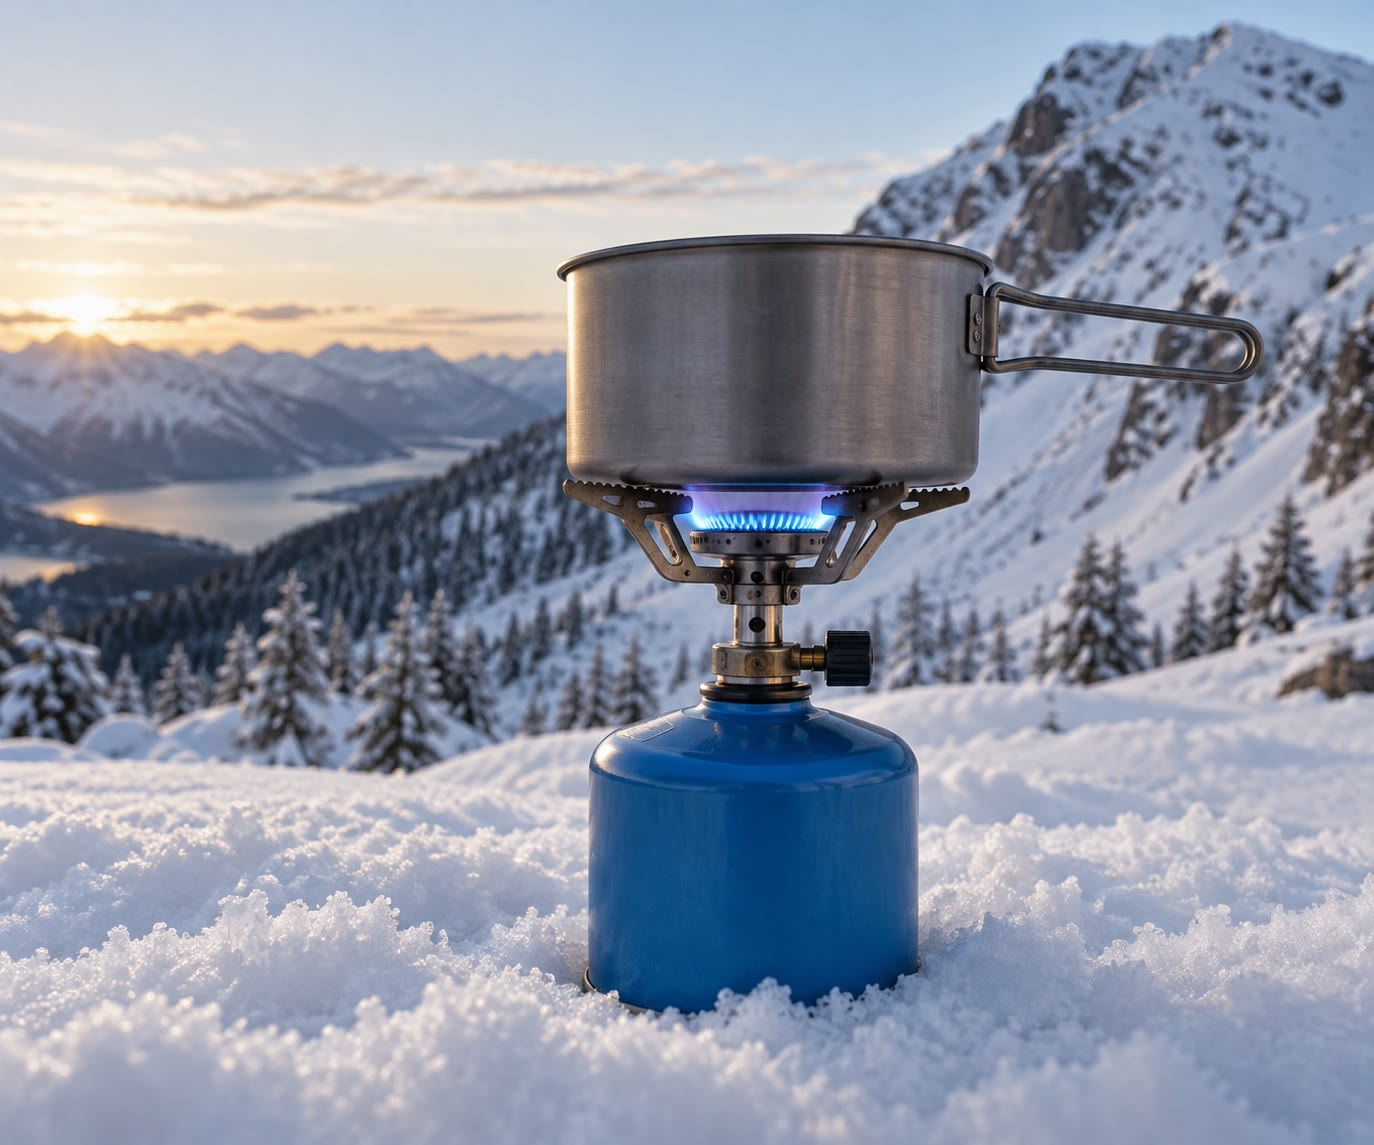
\includegraphics[width=0.48\linewidth]{images/book1/ai/g11-camping-cartridge.jpg}

{\small A camping stove in the snow, \omterm{def:g4:what-a-fire-needs:burning}{burning} a gas made of carbon and
hydrogen.}
\end{omfigure}

\section{Formulas of organic molecules}

\begin{definition}[Organic compound]\label{def:g11:organic-skeletons:organic}
An \emph{organic compound}\index{organic compound} is a compound whose
\omterm{def:g7:atoms-and-molecules:molecule}{molecules} are built on a skeleton of carbon \omterm{def:g7:atoms-and-molecules:atom}{atoms} bonded to one another
and to hydrogen \omterm{def:g7:atoms-and-molecules:atom}{atoms}, possibly with other \omterm{def:g7:atoms-and-molecules:atom}{atoms} such as oxygen and
nitrogen. (Carbon dioxide, carbon monoxide and the carbonates are
traditionally left out.)
\end{definition}

\begin{definition}[Four kinds of formula]\label{def:g11:organic-skeletons:formulas}
A \omterm{def:g7:atoms-and-molecules:molecule}{molecule} can be written in four ways:
\begin{itemize}
  \item its \emph{molecular formula}\index{molecular formula} gives only
        the number of \omterm{def:g7:atoms-and-molecules:atom}{atoms} of each element, such as \ce{C4H10};
  \item its \emph{structural formula}\index{structural formula} shows
        every \omterm{def:g7:atoms-and-molecules:atom}{atom} and every bond;
  \item its \emph{semi-structural formula}\index{semi-structural formula}
        shows the bonds between carbon \omterm{def:g7:atoms-and-molecules:atom}{atoms} and groups the hydrogen
        \omterm{def:g7:atoms-and-molecules:atom}{atoms} with their carbon, such as \ce{CH3-CH2-CH2-CH3};
  \item its \emph{skeletal formula}\index{skeletal formula} draws only
        the bonds of the carbon skeleton as a zigzag: each end and each
        corner is a carbon \omterm{def:g7:atoms-and-molecules:atom}{atom}, the hydrogen \omterm{def:g7:atoms-and-molecules:atom}{atoms} on carbon are not
        drawn, and every other \omterm{def:g7:atoms-and-molecules:atom}{atom} (with its hydrogen \omterm{def:g7:atoms-and-molecules:atom}{atoms}) is written.
\end{itemize}
\end{definition}

\begin{omfigure}
\setchemfig{atom sep=1.45em}
\renewcommand{\arraystretch}{1.6}
\small
\begin{tabular}{@{}l@{\quad}c@{\quad}c@{}}
 & butane & 2-methylpropane \\
molecular & \ce{C4H10} & \ce{C4H10} \\[4pt]
structural &
\chemfig{H-C(-[2]H)(-[6]H)-C(-[2]H)(-[6]H)-C(-[2]H)(-[6]H)-C(-[2]H)(-[6]H)-H} &
\chemfig{H-C(-[2]H)(-[6]H)-C(-[6]H)(-[2,1.5]C(-[1]H)(-[3]H)(-[2]H))-C(-[2]H)(-[6]H)-H} \\[10pt]
semi-structural & \ce{CH3-CH2-CH2-CH3} &
\chemfig{CH_3-CH(-[6]CH_3)-CH_3} \\[14pt]
skeletal & \chemfig{-[:30]-[:-30]-[:30]} & \chemfig{-[:30](-[:90])-[:-30]} \\
\end{tabular}

{\small The four formulas of butane and of 2-methylpropane. In the
\omterm{def:g11:organic-skeletons:formulas}{skeletal formulas}, each end and each corner of the lines is a carbon
\omterm{def:g7:atoms-and-molecules:atom}{atom}: four in each.}
\end{omfigure}


\begin{example}[Reading a skeletal formula]\label{ex:g11:organic-skeletons:reading}
In the \omterm{def:g11:organic-skeletons:formulas}{skeletal formula} of butane, the zigzag has two ends and two
corners: four carbon \omterm{def:g7:atoms-and-molecules:atom}{atoms}. Each end carbon has one bond drawn, so it
carries three hydrogen \omterm{def:g7:atoms-and-molecules:atom}{atoms} (\ce{CH3}); each corner has two bonds drawn,
so it carries two (\ce{CH2}). Every carbon has four bonds in all, which
gives back \ce{C4H10}.
\end{example}

\section{Carbon chains}

The carbon skeleton of a \omterm{def:g7:atoms-and-molecules:molecule}{molecule} can be a \emph{linear} chain, each
carbon bonded to at most two others, as in butane; a \emph{branched}
chain, with at least one carbon bonded to three or four others, as in
2-methylpropane; or a \emph{ring}, as in cyclohexane, \ce{C6H12}, whose
\omterm{def:g11:organic-skeletons:formulas}{skeletal formula} is a hexagon. A zigzag is used for chains because the
real bonds around each carbon make angles of about \ang{109.5}, not
\ang{180}: a ``linear'' chain is in fact a zigzag in space.

\begin{omfigure}
\setchemfig{atom sep=1.9em}
\begin{tabular}{ccc}
\chemfig{-[:30]-[:-30]-[:30]-[:-30]-[:30]} &
\chemfig{-[:30](-[:90])-[:-30]-[:30](-[:90])-[:-30]} &
\chemfig{*6(------)} \\[4pt]
\small linear: hexane & \small branched: 2,4-dimethylpentane &
\small ring: cyclohexane \\
\small \ce{C6H14} & \small \ce{C7H16} & \small \ce{C6H12}
\end{tabular}

{\small Three carbon skeletons, in \omterm{def:g11:organic-skeletons:formulas}{skeletal formulas}.}
\end{omfigure}

\section{Alkanes and their names}

\begin{definition}[Alkane, alkyl group]\label{def:g11:organic-skeletons:alkane}
An \emph{alkane}\index{alkane} is a compound of carbon and hydrogen whose
skeleton is a chain (linear or branched, not a ring) with only single
bonds; its \omterm{def:g11:organic-skeletons:formulas}{molecular formula} is \ce{C_{n}H_{2n+2}}. An \emph{alkyl
group}\index{alkyl group} is what remains of an alkane when one hydrogen
\omterm{def:g7:atoms-and-molecules:atom}{atom} is removed, so that it can be attached to a chain: methyl
\ce{-CH3}, ethyl \ce{-CH2-CH3}.
\end{definition}

\begin{omfigure}
\begin{tabular}{rlcrlc}
\hline
$n$ & name & formula & $n$ & name & formula \\
\hline
1 & methane & \ce{CH4}    & 6  & hexane & \ce{C6H14} \\
2 & ethane  & \ce{C2H6}   & 7  & heptane & \ce{C7H16} \\
3 & propane & \ce{C3H8}   & 8  & octane & \ce{C8H18} \\
4 & butane  & \ce{C4H10}  & 9  & nonane & \ce{C9H20} \\
5 & pentane & \ce{C5H12}  & 10 & decane & \ce{C10H22} \\
\hline
\end{tabular}\par\medskip

{\small The first ten linear \omterm{def:g11:organic-skeletons:alkane}{alkanes}. The name of a chain of $n$ carbon
\omterm{def:g7:atoms-and-molecules:atom}{atoms} is the same root followed by \emph{-ane}; the \omterm{def:g11:organic-skeletons:alkane}{alkyl group}
replaces \emph{-ane} by \emph{-yl} (methyl, ethyl, propyl\dots).}
\end{omfigure}

\begin{method}[Naming an alkane]\label{met:g11:organic-skeletons:naming}
\begin{enumerate}
  \item Find the longest chain of carbon \omterm{def:g7:atoms-and-molecules:atom}{atoms}: it gives the root name
        (pentane, hexane\dots).
  \item The \omterm{def:g7:atoms-and-molecules:atom}{atoms} not in it form \omterm{def:g11:organic-skeletons:alkane}{alkyl groups} attached to it, the
        substituents.
  \item Number the main chain from the end that gives the substituents
        the lowest numbers.
  \item Write each substituent with its number (its position on the
        chain), in alphabetical order, before the root; repeated groups
        take the prefixes di-, tri-, tetra-, with one number each.
        Numbers are separated by commas, numbers and words by hyphens.
\end{enumerate}
\end{method}

\begin{omfigure}
\begin{tikzpicture}[font=\small, x=0.9cm, y=0.9cm]
  % main chain of 5, zigzag; methyls on C2 and C3
  \coordinate (a1) at (0,0); \coordinate (a2) at (0.87,0.5);
  \coordinate (a3) at (1.73,0); \coordinate (a4) at (2.6,0.5);
  \coordinate (a5) at (3.46,0);
  \coordinate (m2) at (0.87,1.5); \coordinate (m3) at (1.73,-1);
  \draw[line width=1pt] (a1) -- (a2) -- (a3) -- (a4) -- (a5);
  \draw[line width=1pt] (a2) -- (m2); \draw[line width=1pt] (a3) -- (m3);
  \foreach \k in {1,2,3,4,5}
    \node[omDef, font=\footnotesize\bfseries, fill=white, inner sep=1pt]
      at ($(a\k)+(0,-0.32)$) {\k};
  \draw[omProp, thick] (m2) circle (0.28);
  \draw[omProp, thick] (m3) circle (0.28);
  \node[omProp, anchor=west] at ($(m2)+(0.35,0)$) {methyl on C2};
  \node[omProp, anchor=west] at ($(m3)+(0.35,0)$) {methyl on C3};
  \node[anchor=west, align=left] at (5,0.3) {longest chain: 5 carbons,
    \emph{pentane}\\ numbered from the left: 2 and 3\\ (from the right: 3
    and 4, higher)\\ name: \textbf{2,3-dimethylpentane}};
\end{tikzpicture}

{\small Naming a branched \omterm{def:g11:organic-skeletons:alkane}{alkane}: the main chain (numbered), the
substituents (circled), the name.}
\end{omfigure}

\begin{method}[From a name to a skeletal formula]\label{met:g11:organic-skeletons:drawing}
\begin{enumerate}
  \item Draw the main chain given by the root, as a zigzag, and number
        its carbons.
  \item Attach each substituent at the position given by its number.
  \item Check: count the carbons, and that no carbon has more than four
        bonds.
\end{enumerate}
\end{method}

\section{Isomers}

\begin{definition}[Isomers, constitutional isomers]\label{def:g11:organic-skeletons:isomer}
\emph{Isomers}\index{isomers} are different compounds with the same
\omterm{def:g11:organic-skeletons:formulas}{molecular formula}. \emph{Constitutional isomers}\index{constitutional
isomers} are isomers whose \omterm{def:g7:atoms-and-molecules:atom}{atoms} are bonded in a different order, for
example with a different carbon skeleton.
\end{definition}

\begin{proposition}[Isomers have different properties]\label{prop:g11:organic-skeletons:properties}
% ledger: bp:C4H10, bp:isobutane, bp:C5H12, bp:isopentane, bp:neopentane
\omterm{def:g11:organic-skeletons:isomer}{Constitutional isomers} are different substances, with different
properties. Among the \omterm{def:g11:organic-skeletons:alkane}{alkane} \omterm{def:g11:organic-skeletons:isomer}{isomers} of a given formula, the more
branched ones boil lower: butane boils near \qty{0}{\celsius} and
2-methylpropane at \qty{-11.7}{\celsius}; pentane at
\qty{36.1}{\celsius}, 2-methylbutane at \qty{27.8}{\celsius} and
2,2-dimethylpropane at \qty{9.5}{\celsius}.
\end{proposition}

\begin{proof}
The values are measured (ledger). Branched \omterm{def:g7:atoms-and-molecules:molecule}{molecules} are more compact,
with less surface in contact with their neighbours: their \omterm{def:g11:polarity-and-cohesion:van-der-waals}{van der Waals
interactions} are weaker (\cref{ch:g11:polarity-and-cohesion}).
\end{proof}

\begin{omfigure}
\setchemfig{atom sep=2em}
\begin{tabular}{ccc}
\chemfig{-[:30]-[:-30]-[:30]-[:-30]} &
\chemfig{-[:30](-[:90])-[:-30]-[:30]} &
\chemfig{-[:0](-[:90])(-[:-90])-[:0]} \\[24pt]
\small pentane & \small 2-methylbutane & \small 2,2-dimethylpropane \\
\small \qty{36.1}{\celsius} & \small \qty{27.8}{\celsius} &
\small \qty{9.5}{\celsius}
\end{tabular}
\medskip

{\small The three \omterm{def:g11:organic-skeletons:isomer}{isomers} of \ce{C5H12} and their boiling temperatures:
the more branched, the lower.}
\end{omfigure}

\section{Alkanes from crude oil}

Crude oil is a \omterm{def:g6:pure-substances-and-mixtures:mixture}{mixture} of thousands of compounds, most of them \omterm{def:g11:organic-skeletons:alkane}{alkanes}
with 1 to more than 40 carbon \omterm{def:g7:atoms-and-molecules:atom}{atoms}. In a refinery it is heated and its
vapours rise through a tall column, cooler and cooler towards the top:
each fraction condenses at the height where the temperature matches its
boiling range. Gases (methane to butane) leave at the top, then petrol,
kerosene, diesel; heavy oils and bitumen stay at the bottom. This
fractional \omterm{def:g10:chemical-species:distillation}{distillation} separates by boiling temperature, which for
\omterm{def:g11:organic-skeletons:alkane}{alkanes} grows with the length of the chain.

\begin{omfigure}
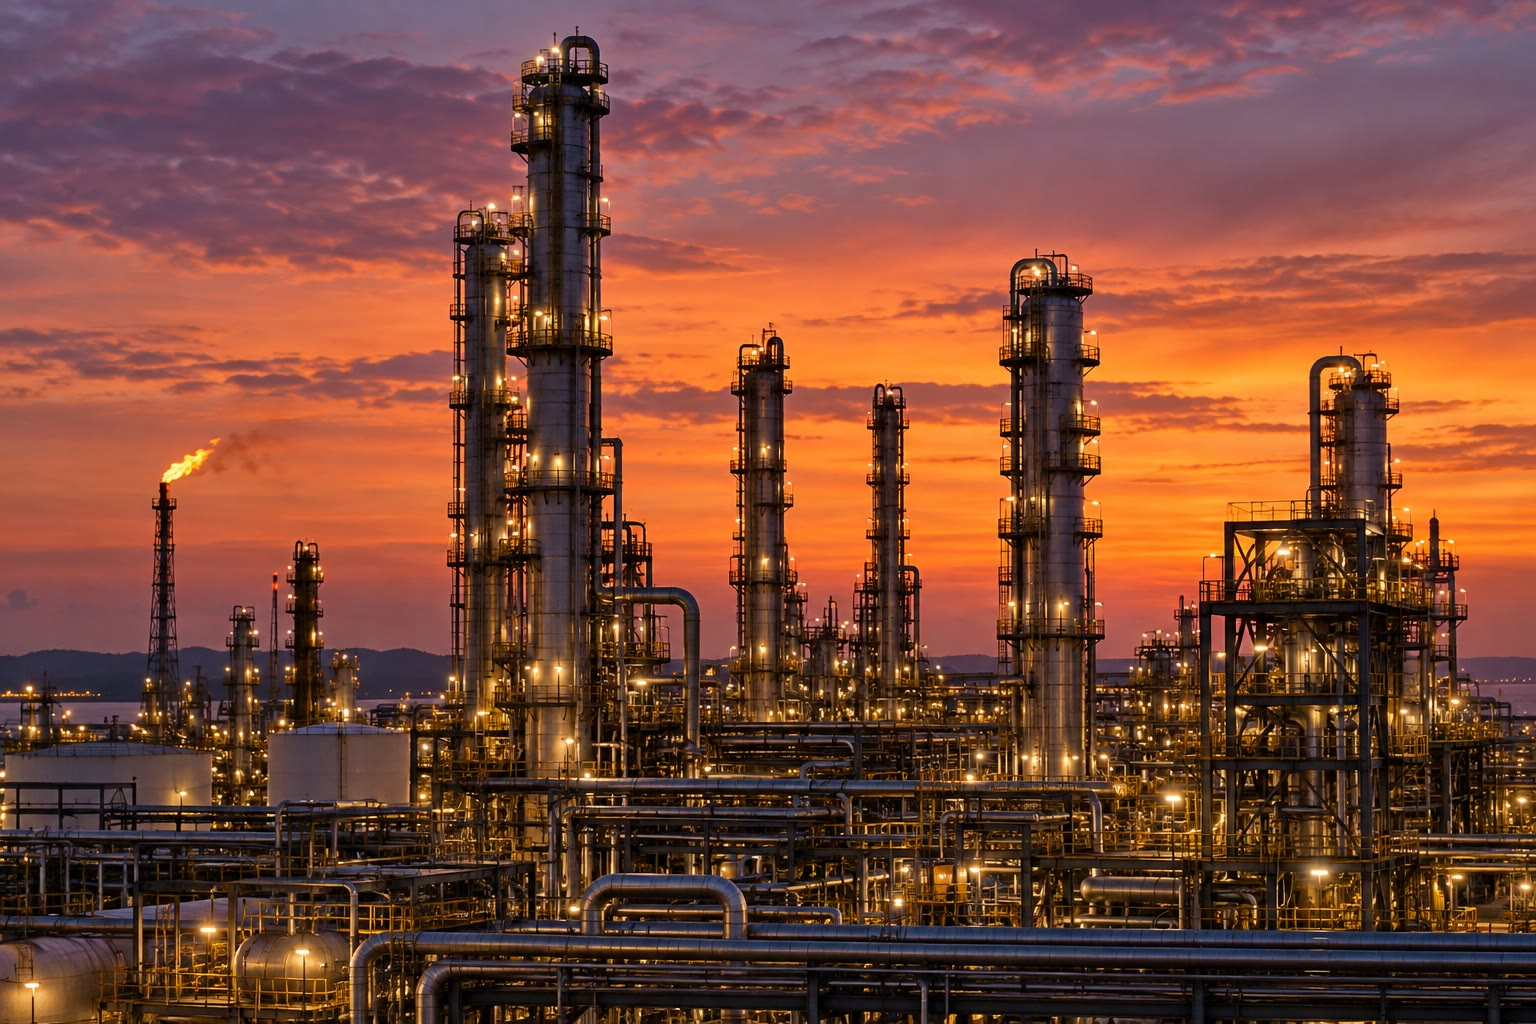
\includegraphics[width=0.52\linewidth]{images/book1/ai/g11-refinery-dusk.jpg}

{\small \omterm{def:g10:chemical-species:distillation}{Distillation} columns of a refinery at dusk.}
\end{omfigure}

\begin{safety}{\ghs[0.66cm]{GHS02}\ghs[0.66cm]{GHS04}\ghs[0.66cm]{GHS07}\ghs[0.66cm]{GHS08}\ghs[0.66cm]{GHS09}}
% ledger: ghs:butane, ghs:pentane
Butane is an extremely flammable gas, stored under pressure. Pentane is
a highly flammable liquid; its vapour causes drowsiness, it can damage
the lungs if swallowed and it is toxic to aquatic life. No flame near
light \omterm{def:g11:organic-skeletons:alkane}{alkanes}; work under a fume hood.
\end{safety}

\section{Exercises}


\begin{exercise}[$\star$]\label{exo:g11:organic-skeletons:1}
Give the \omterm{def:g11:organic-skeletons:formulas}{molecular formulas} of the \omterm{def:g7:atoms-and-molecules:molecule}{molecules} drawn here, and say whether
they are \omterm{def:g11:organic-skeletons:isomer}{isomers}:
\setchemfig{atom sep=1.6em}
\chemfig{-[:30]-[:-30]-[:30]-[:-30]-[:30]} \quad and \quad
\chemfig{-[:30](-[:90])-[:-30]-[:30]-[:-30]}.
\end{exercise}

\begin{exercise}[$\star$]\label{exo:g11:organic-skeletons:2}
Name: \ce{CH3-CH2-CH3}; \ce{CH3-CH2-CH2-CH2-CH2-CH3};
\chemfig{CH_3-CH(-[2]CH_3)-CH_2-CH_3}.
\end{exercise}

\begin{exercise}[$\star$]\label{exo:g11:organic-skeletons:3}
Write the \omterm{def:g11:organic-skeletons:formulas}{semi-structural formulas} of propane and of 2-methylpropane, and
the \omterm{def:g11:organic-skeletons:formulas}{structural formula} of ethane.
\end{exercise}

\begin{exercise}[$\star$]\label{exo:g11:organic-skeletons:4}
Count the carbon and hydrogen \omterm{def:g7:atoms-and-molecules:atom}{atoms} of each \omterm{def:g7:atoms-and-molecules:molecule}{molecule}:
\setchemfig{atom sep=1.6em}
\chemfig{-[:30]-[:-30](-[:-90])-[:30]-[:-30]} \quad and \quad
\chemfig{*6(------)}.
\end{exercise}

\begin{exercise}[$\star$]\label{exo:g11:organic-skeletons:5}
Give the \omterm{def:g11:organic-skeletons:formulas}{molecular formula} of the \omterm{def:g11:organic-skeletons:alkane}{alkane} with 8 carbon \omterm{def:g7:atoms-and-molecules:atom}{atoms}, and the
number of carbon \omterm{def:g7:atoms-and-molecules:atom}{atoms} of the \omterm{def:g11:organic-skeletons:alkane}{alkane} with 20 hydrogen \omterm{def:g7:atoms-and-molecules:atom}{atoms}.
\end{exercise}

\begin{exercise}[$\star\star$]\label{exo:g11:organic-skeletons:6}
Draw the \omterm{def:g11:organic-skeletons:formulas}{skeletal formulas} of 3-methylhexane, 2,2-dimethylbutane and
3-ethylpentane, and give their \omterm{def:g11:organic-skeletons:formulas}{molecular formulas}.
\end{exercise}

\begin{exercise}[$\star\star$]\label{exo:g11:organic-skeletons:7}
Draw and name the three \omterm{def:g11:organic-skeletons:isomer}{isomers} of \ce{C5H12}.
\end{exercise}

\begin{exercise}[$\star\star$]\label{exo:g11:organic-skeletons:8}
These names are wrong. Draw each \omterm{def:g7:atoms-and-molecules:molecule}{molecule} and give its correct name:
2-ethylbutane; 4-methylpentane; 1-methylbutane.
\end{exercise}

\begin{exercise}[$\star\star$]\label{exo:g11:organic-skeletons:9}
Using the figure of the \omterm{def:g11:organic-skeletons:isomer}{isomers} of \ce{C5H12}, rank them by boiling
temperature and explain the order.
\end{exercise}

\begin{exercise}[$\star\star$]\label{exo:g11:organic-skeletons:10}
Cyclohexane is \ce{C6H12} and hexane \ce{C6H14}. Explain the two
missing hydrogen \omterm{def:g7:atoms-and-molecules:atom}{atoms}. Are the two compounds \omterm{def:g11:organic-skeletons:isomer}{isomers}? Is cyclohexane an
\omterm{def:g11:organic-skeletons:alkane}{alkane}?
\end{exercise}

\begin{exercise}[$\star\star$]\label{exo:g11:organic-skeletons:11}
Among propane, butane, 2-methylpropane and cyclobutane (\ce{C4H8}, a
ring of four carbon \omterm{def:g7:atoms-and-molecules:atom}{atoms}), which are \omterm{def:g11:organic-skeletons:isomer}{isomers} of one another?
\end{exercise}

\begin{exercise}[$\star\star\star$]\label{exo:g11:organic-skeletons:12}
Draw and name the five \omterm{def:g11:organic-skeletons:isomer}{isomers} of \ce{C6H14}.
\end{exercise}

\begin{exercise}[$\star\star\star$]\label{exo:g11:organic-skeletons:13}
Picture a linear \omterm{def:g11:organic-skeletons:alkane}{alkane} as a long zigzag and a very branched one as a
ball. Using this picture, explain why branching lowers the boiling
temperature of \omterm{def:g11:organic-skeletons:isomer}{isomers}.
\end{exercise}

\begin{exercise}[$\star\star\star$]\label{exo:g11:organic-skeletons:14}
Name the \omterm{def:g11:organic-skeletons:alkane}{alkane}
\begin{center}
\chemfig{CH_3-CH(-[2]CH_3)-CH_2-C(-[2]CH_3)(-[6]CH_3)-CH_2-CH_3}
\end{center}
\end{exercise}

\begin{exercise}[$\star\star\star$]\label{exo:g11:organic-skeletons:15}
The reference compound for petrol, ``isooctane'', is
2,2,4-trimethylpentane. Draw its \omterm{def:g11:organic-skeletons:formulas}{skeletal formula}, check that it is an
isomer of octane, and write its \omterm{def:g11:organic-skeletons:formulas}{semi-structural formula}.
\end{exercise}

\section{Problem: Lighter Gas}

\begin{problem}[{Weekend problem --- how many different \omterm{def:g11:organic-skeletons:alkane}{alkanes} have the
formula \ce{C7H16}?}]
\label{pb:g11:organic-skeletons:1}
% ledger: bp:C3H8, bp:C4H10, bp:isobutane
A lighter holds butane; a winter camping cartridge holds a blend richer
in propane or in 2-methylpropane. Butane boils at about
\qty{0}{\celsius}, 2-methylpropane at \qty{-11.7}{\celsius} and propane
at \qty{-42}{\celsius}.

\medskip
\noindent\textbf{Part I --- Two gases with one formula.}
\begin{enumerate}
  \item Give the \omterm{def:g11:organic-skeletons:formulas}{molecular formula} of butane, and check that it fits the
        general formula of the \omterm{def:g11:organic-skeletons:alkane}{alkanes}.
  \item Draw its \omterm{def:g11:organic-skeletons:formulas}{structural formula}.
  \item Write its semi-structural and \omterm{def:g11:organic-skeletons:formulas}{skeletal formulas}.
  \item Draw 2-methylpropane in the same three ways. Why does it have
        the same \omterm{def:g11:organic-skeletons:formulas}{molecular formula}?
  \item Are butane and 2-methylpropane \omterm{def:g11:organic-skeletons:isomer}{isomers}? Of which kind?
\end{enumerate}

\medskip
\noindent\textbf{Part II --- In the cold.}
\begin{enumerate}[resume]
  \item Which of the three gases are gases at \qty{20}{\celsius} and
        normal pressure?
  \item An open lighter is used outdoors at \qty{-5}{\celsius}. Why
        does it give a poor flame?
  \item Why are winter cartridges rich in propane or in 2-methylpropane?
  \item Explain why 2-methylpropane boils lower than butane.
  \item Why does propane have no isomer?
\end{enumerate}

\medskip
\noindent\textbf{Part III --- Naming and counting.}
\begin{enumerate}[resume]
  \item Name \chemfig{CH_3-CH(-[2]CH_3)-CH_2-CH_3}.
  \item Why is the name ``3-methylbutane'' wrong for the same \omterm{def:g7:atoms-and-molecules:molecule}{molecule}?
  \item How many \omterm{def:g11:organic-skeletons:alkane}{alkane} \omterm{def:g11:organic-skeletons:isomer}{isomers} have the formulas \ce{C4H10},
        \ce{C5H12} and \ce{C6H14}?
\end{enumerate}

\medskip
\noindent\textbf{Part IV --- The \omterm{def:g11:organic-skeletons:isomer}{isomers} of \ce{C7H16}.}
\begin{enumerate}[resume]
  \item Draw the linear isomer and name it.
  \item Draw and name the \omterm{def:g11:organic-skeletons:isomer}{isomers} whose longest chain has six carbon
        \omterm{def:g7:atoms-and-molecules:atom}{atoms}. Why is there no ``4-methylhexane''?
  \item Draw and name the \omterm{def:g11:organic-skeletons:isomer}{isomers} whose longest chain has five carbon
        \omterm{def:g7:atoms-and-molecules:atom}{atoms} and two methyl groups.
  \item Is there an isomer with a five-carbon chain and an ethyl group?
        Why can the ethyl group only sit on carbon 3?
  \item Draw and name the isomer whose longest chain has four carbon
        \omterm{def:g7:atoms-and-molecules:atom}{atoms}.
  \item Count all the \omterm{def:g11:organic-skeletons:isomer}{isomers} found.
  \item State the final answer: how many \omterm{def:g11:organic-skeletons:isomer}{constitutional isomers} does
        heptane have, itself included?
\end{enumerate}
\end{problem}
